\section{力的测量}\label{sec:2-4}

力的大小可以用仪器来测量,测量力的仪器叫做测力计。测力计的种类很多,其中常用的一种叫弹簧秤(图 \ref{fig:2-7})。
在图 \ref{fig:2-7} 甲所示的弹簧秤的壳子里有一根钢制的弹簧,弹簧的上端挂在一个圆环上,下端连着一个有刻度的圆柱,柱的下端有钩。
提住上端的圆坏,把物体挂在下端的钩上,弹簧伸长,圆柱随着下降,从柱上露出的刻度就可以读出物重来。
用手拉弹簧秤时,从圆柱上露出的刻度就可以知道手的拉力。
图 \ref{fig:2-7} 乙是另一种形式的弹簧秤,这种弹簧秤的刻度标在外壳上,弹簧下端附有指针,从指针的位置可以读出力的大小。

\begin{figure}[htbp]
    \centering
    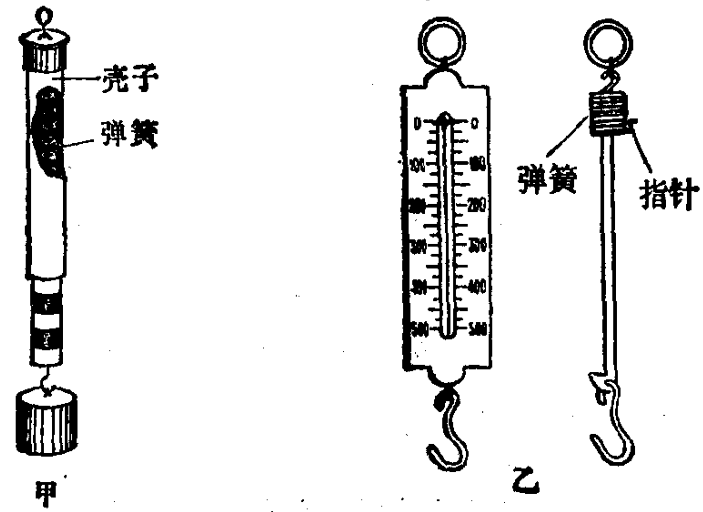
\includegraphics[width=0.5\textwidth]{../pic/czwl1-ch2-7}
    \caption{弹簧称}\label{fig:2-7}
\end{figure}

弹簧秤为什么能够测量力的大小呢?为了弄清这个问题我们来做下面的实验。

\begin{figure}[htbp]
    \centering
    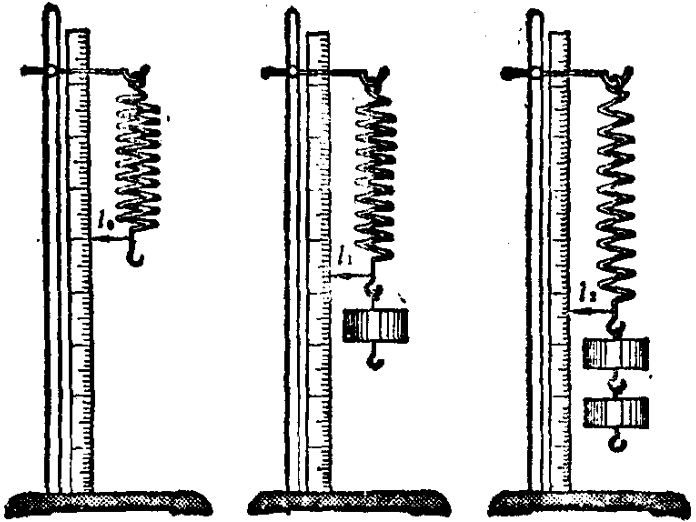
\includegraphics[width=0.5\textwidth]{../pic/czwl1-ch2-8}
    \caption{弹簧伸长的长度跟拉力成正比}\label{fig:2-8}
\end{figure}

象图 \ref{fig:2-8} 那样,在铁架台上固定一根直尺,把下端附有指针的弹簧挂在铁架上,记下这时指针在直尺上指示的位置 $l_0$。
然后把几个质量相等(因而重也相等)的钩码依次在弹簧秤上,先挂一个,再增至两个,三个 ……  每次都记下指针的位置
$l_1$,$l_2$,$l_3$ ……  求出各次弹簧伸长的长度 $\Delta l_1 \footnotemark = l_1 - l_0$,
$\Delta l_2 = l_2 - l_0$,
$\Delta l_3 = l_3 - l_0$ ……
把各次悬挂的钩码重和对应的弹簧伸长的长度列成表。研究弹簧的伸长跟钩码重的关系。下面是一次实验的记录。
\footnotetext{$\Delta$:希腊字母,汉语拼音读法是 delta 。 $\Delta$ 加在物理量的符号前面用来表示物理量的变化。}

\begin{table}[H]
    \centering
    \renewcommand\arraystretch{1.5}
    \begin{tabular}{|w{c}{11em}|*{5}{w{c}{4em}|}}
        \hline
        钩码重 $mg$ (牛顿) & $0.49$ & $0.98$ & $1.47$ & $1.96$ & $2.45$  \\ \hline
        弹簧的伸长 $\Delta l$(厘米) & 2 & 4 & 6 & 8 & 10 \\ \hline
    \end{tabular}
\end{table}

取下钩码,指针回到原来的位置,表明弹簧恢复到原来的长度。把实验重做几次,每次得到的实验记录都跟上表相同。

上面的实验表明弹簧有这样的性质:受到一定大小的拉力,就伸长一定的长度;拉力增大到几倍,
例如由 $0.49$ 牛顿增大到 2 倍($0.98$ 牛顿)或 3 倍〈$1.47$ 牛顿),弹簧的伸长也由 2 厘米增加到 2 倍(4 厘米)或 3 倍(6 厘米),
即\textbf{弹簧的伸长跟受到的拉力成正比}。弹簧秤就是利用了弹簧的这种性质,从弹簧伸长的长度来知道拉力的大小的。

需要注意,每个弹簧秤都有一定的测量范围,加在弹簧秤上的力不能超过这个范围。
如果加在弹簧秤上的力过大,超过了它的测量范围,弹簧的伸长就不再跟拉力成正比,撒去拉力以后,弹簧也不能再恢复原来的长度,弹簧秤就损坏了。
弹簧秤上的最大刻度就是它的测量范围。

除了弹簧秤以外,还有其它形式的测力计。例如测量手的握力的握力计,测量机车、拖拉机牵引力的牵引测力计(图 \ref{fig:2-9})等。

\begin{figure}[htbp]
    \centering
    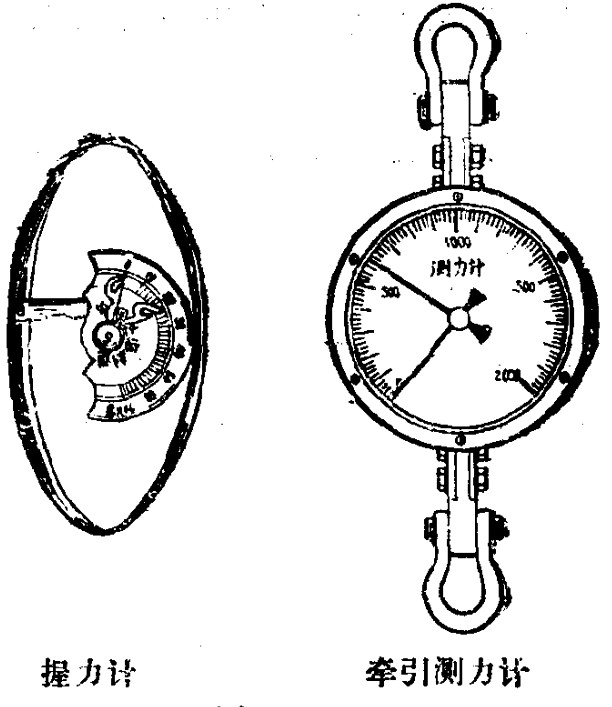
\includegraphics[width=0.4\textwidth]{../pic/czwl1-ch2-9}
    \caption{}\label{fig:2-9}
\end{figure}

